
\section{Methods}

\begin{figure}[tb]
\centering
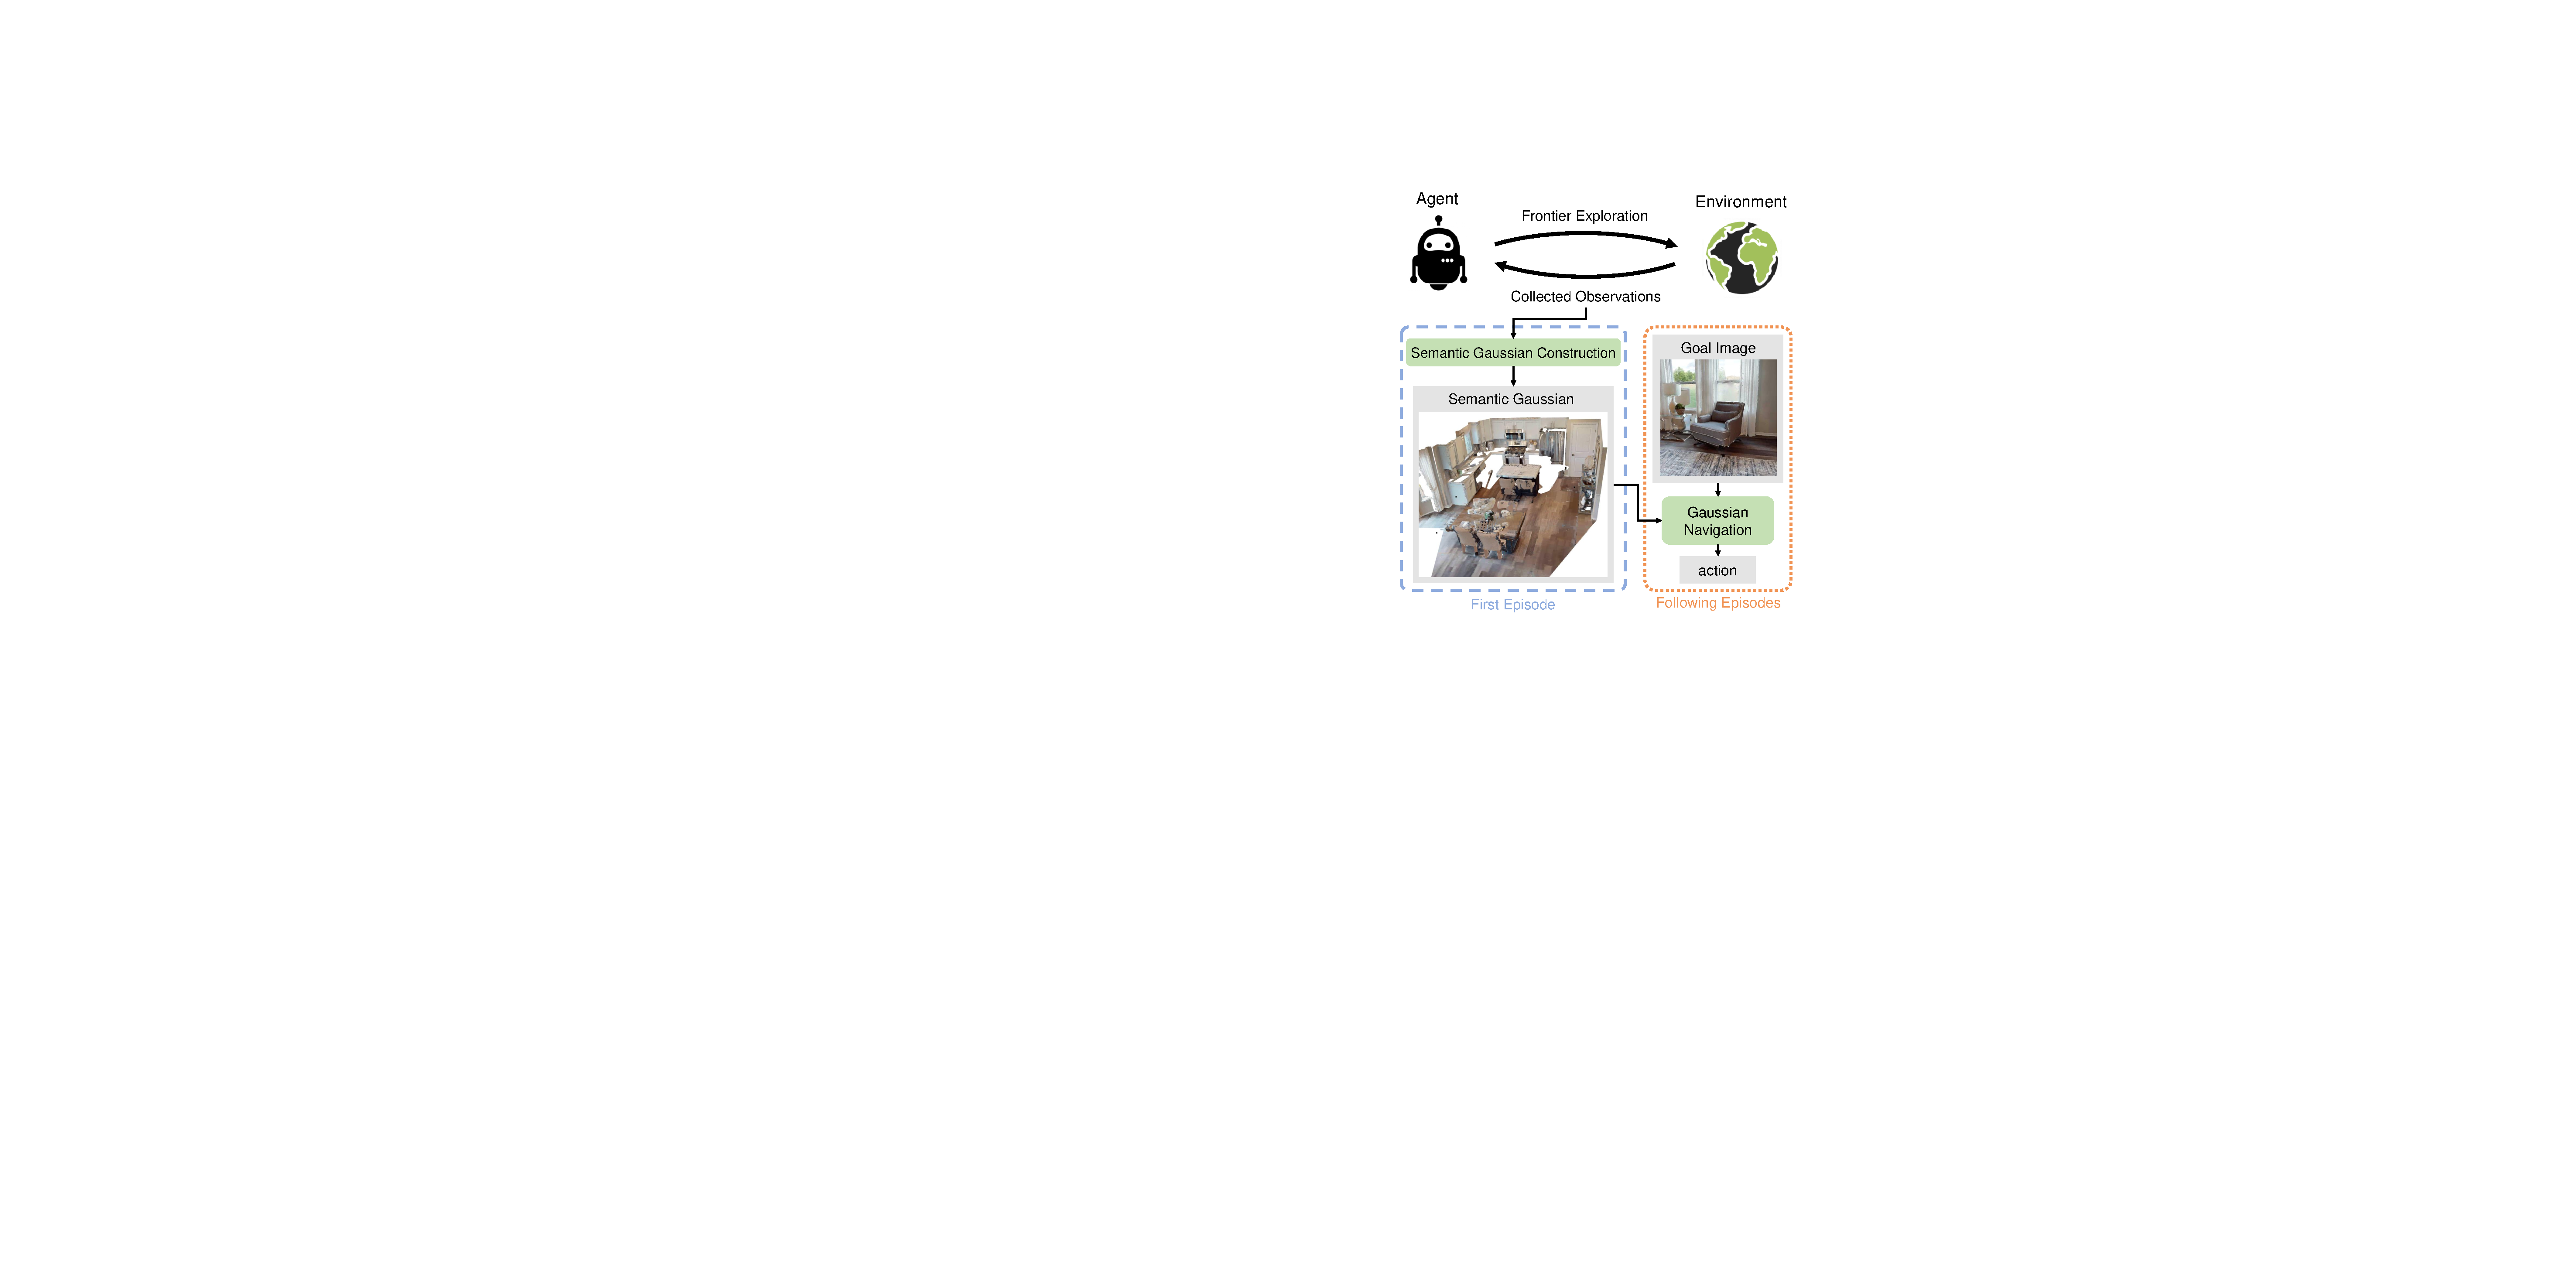
\includegraphics[width=0.95\linewidth]{pics/overview.pdf}
\caption{Framework Overview. In the first episode of a scene, the agent uses frontier exploration to gather observations of the unknown environment, constructing a Semantic Gaussian. In subsequent episodes, the pre-constructed Semantic Gaussian is utilized by Gaussian Navigation to ground the goal object and guide the agent towards it. }
\vspace{-6pt}
\label{fig:framework_overview}
\end{figure}

\begin{figure}[tb]
\centering
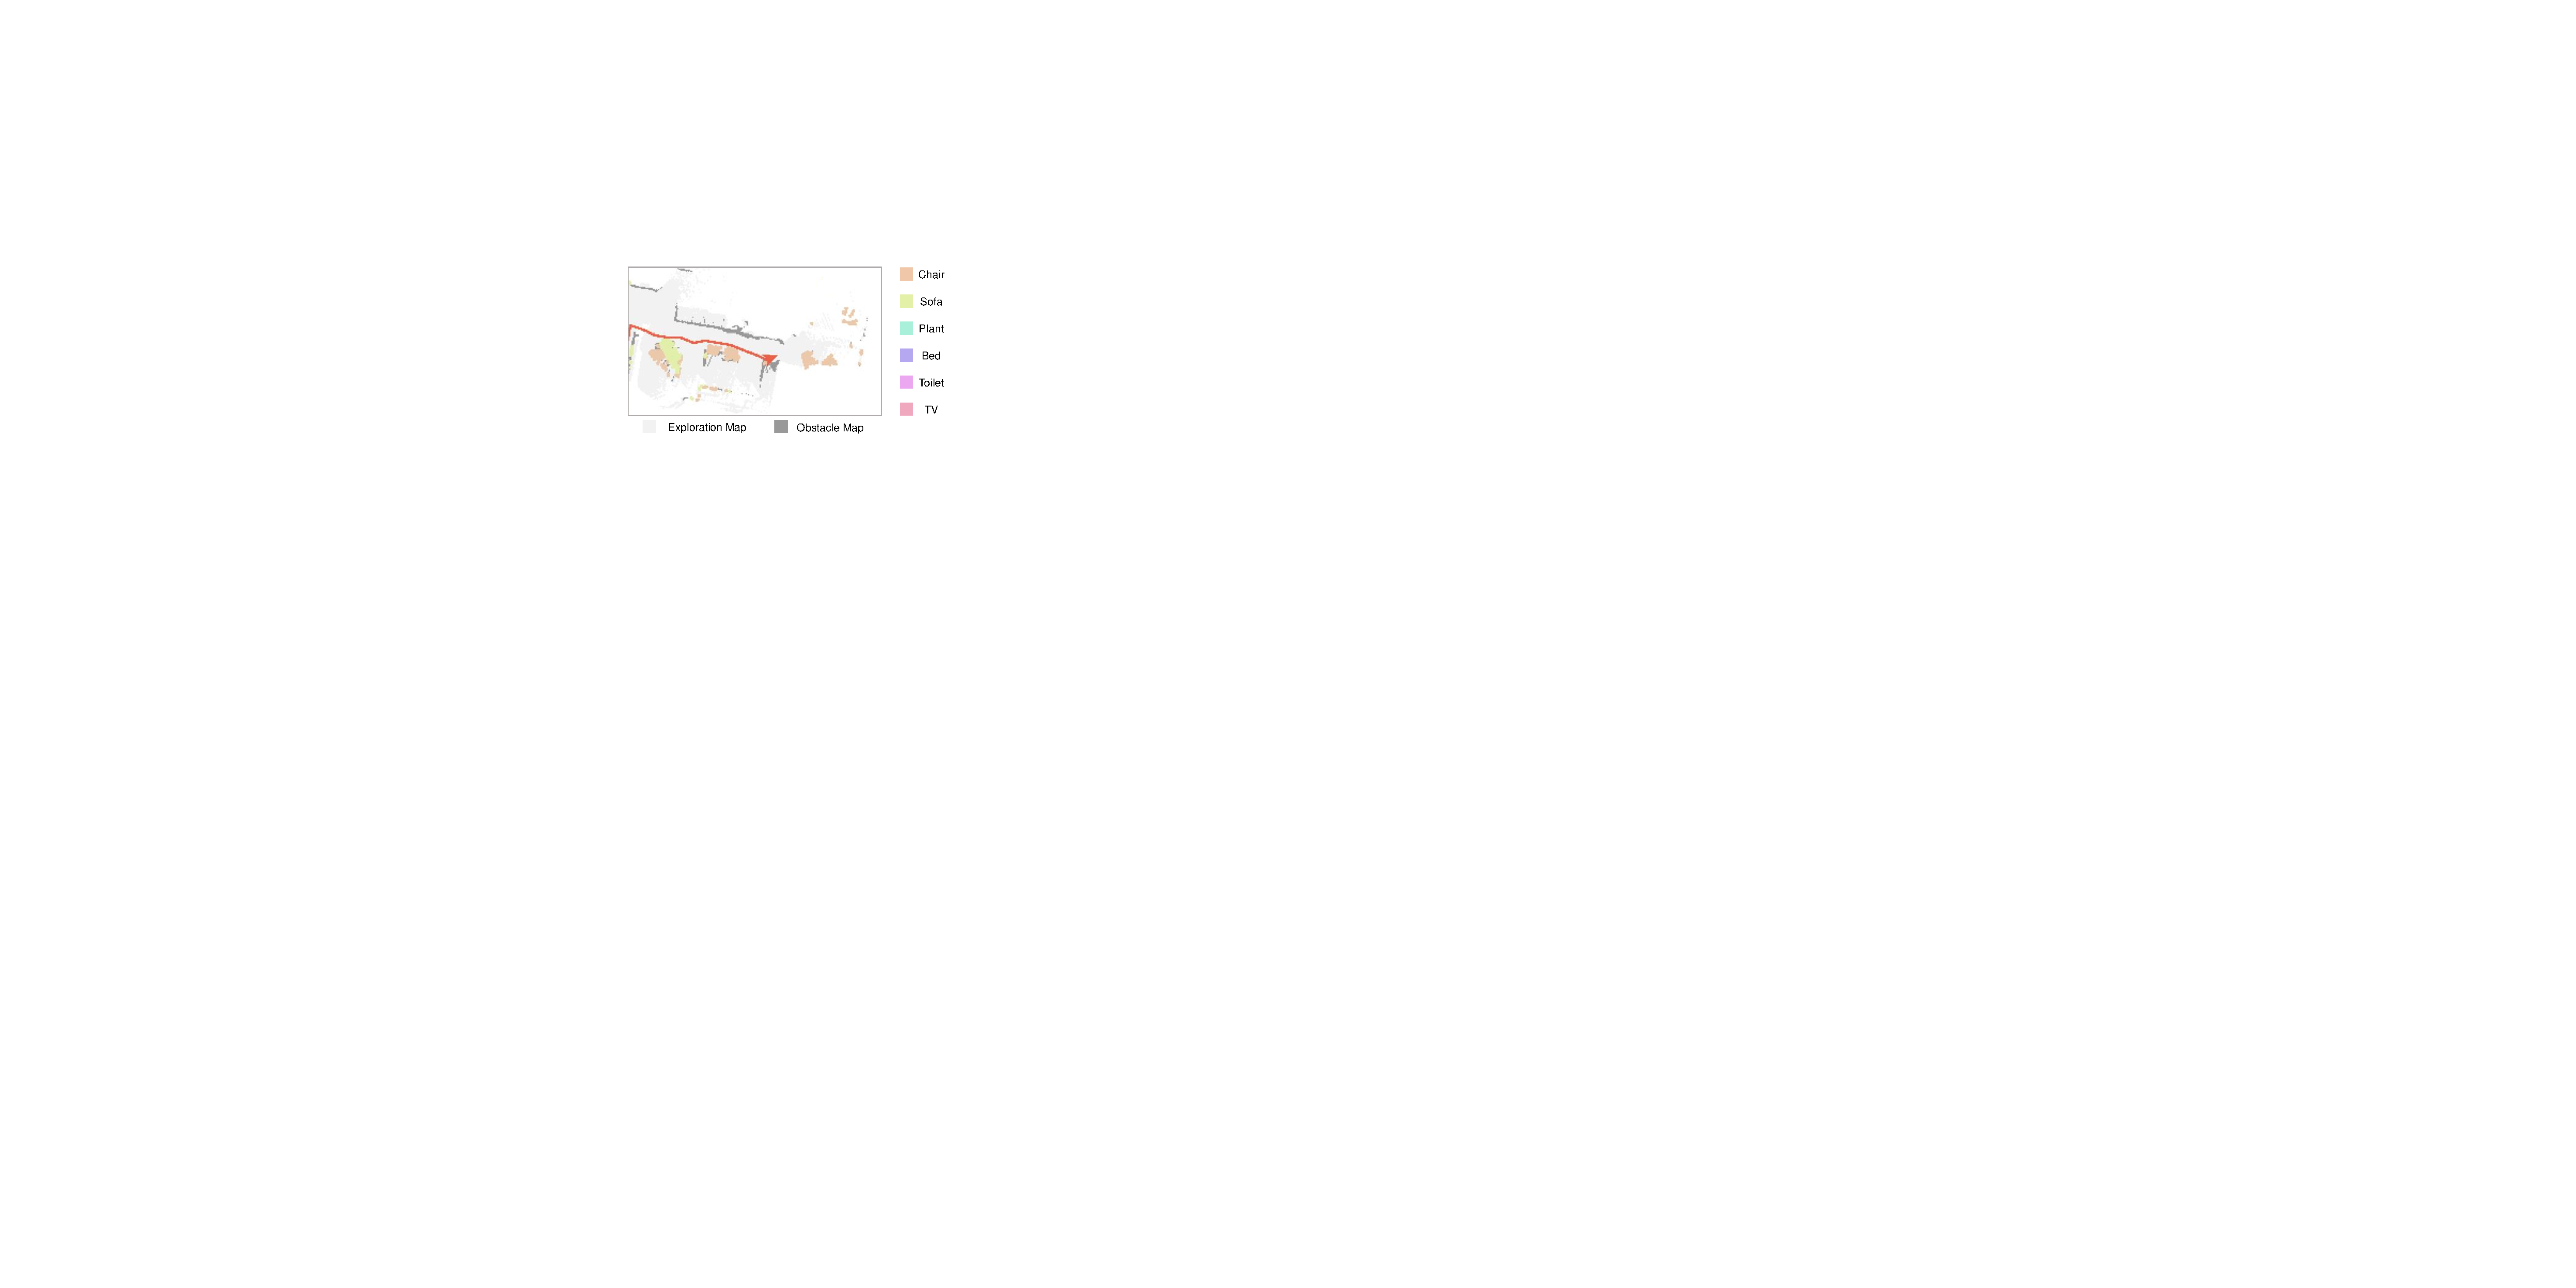
\includegraphics[width=0.98\linewidth]{pics/map.pdf}
\caption{Exploration Map and Obstacle Map.}
\vspace{-16pt}
\label{fig:exp_obs_map}
\end{figure}

% \begin{figure*}
%   \centering
%   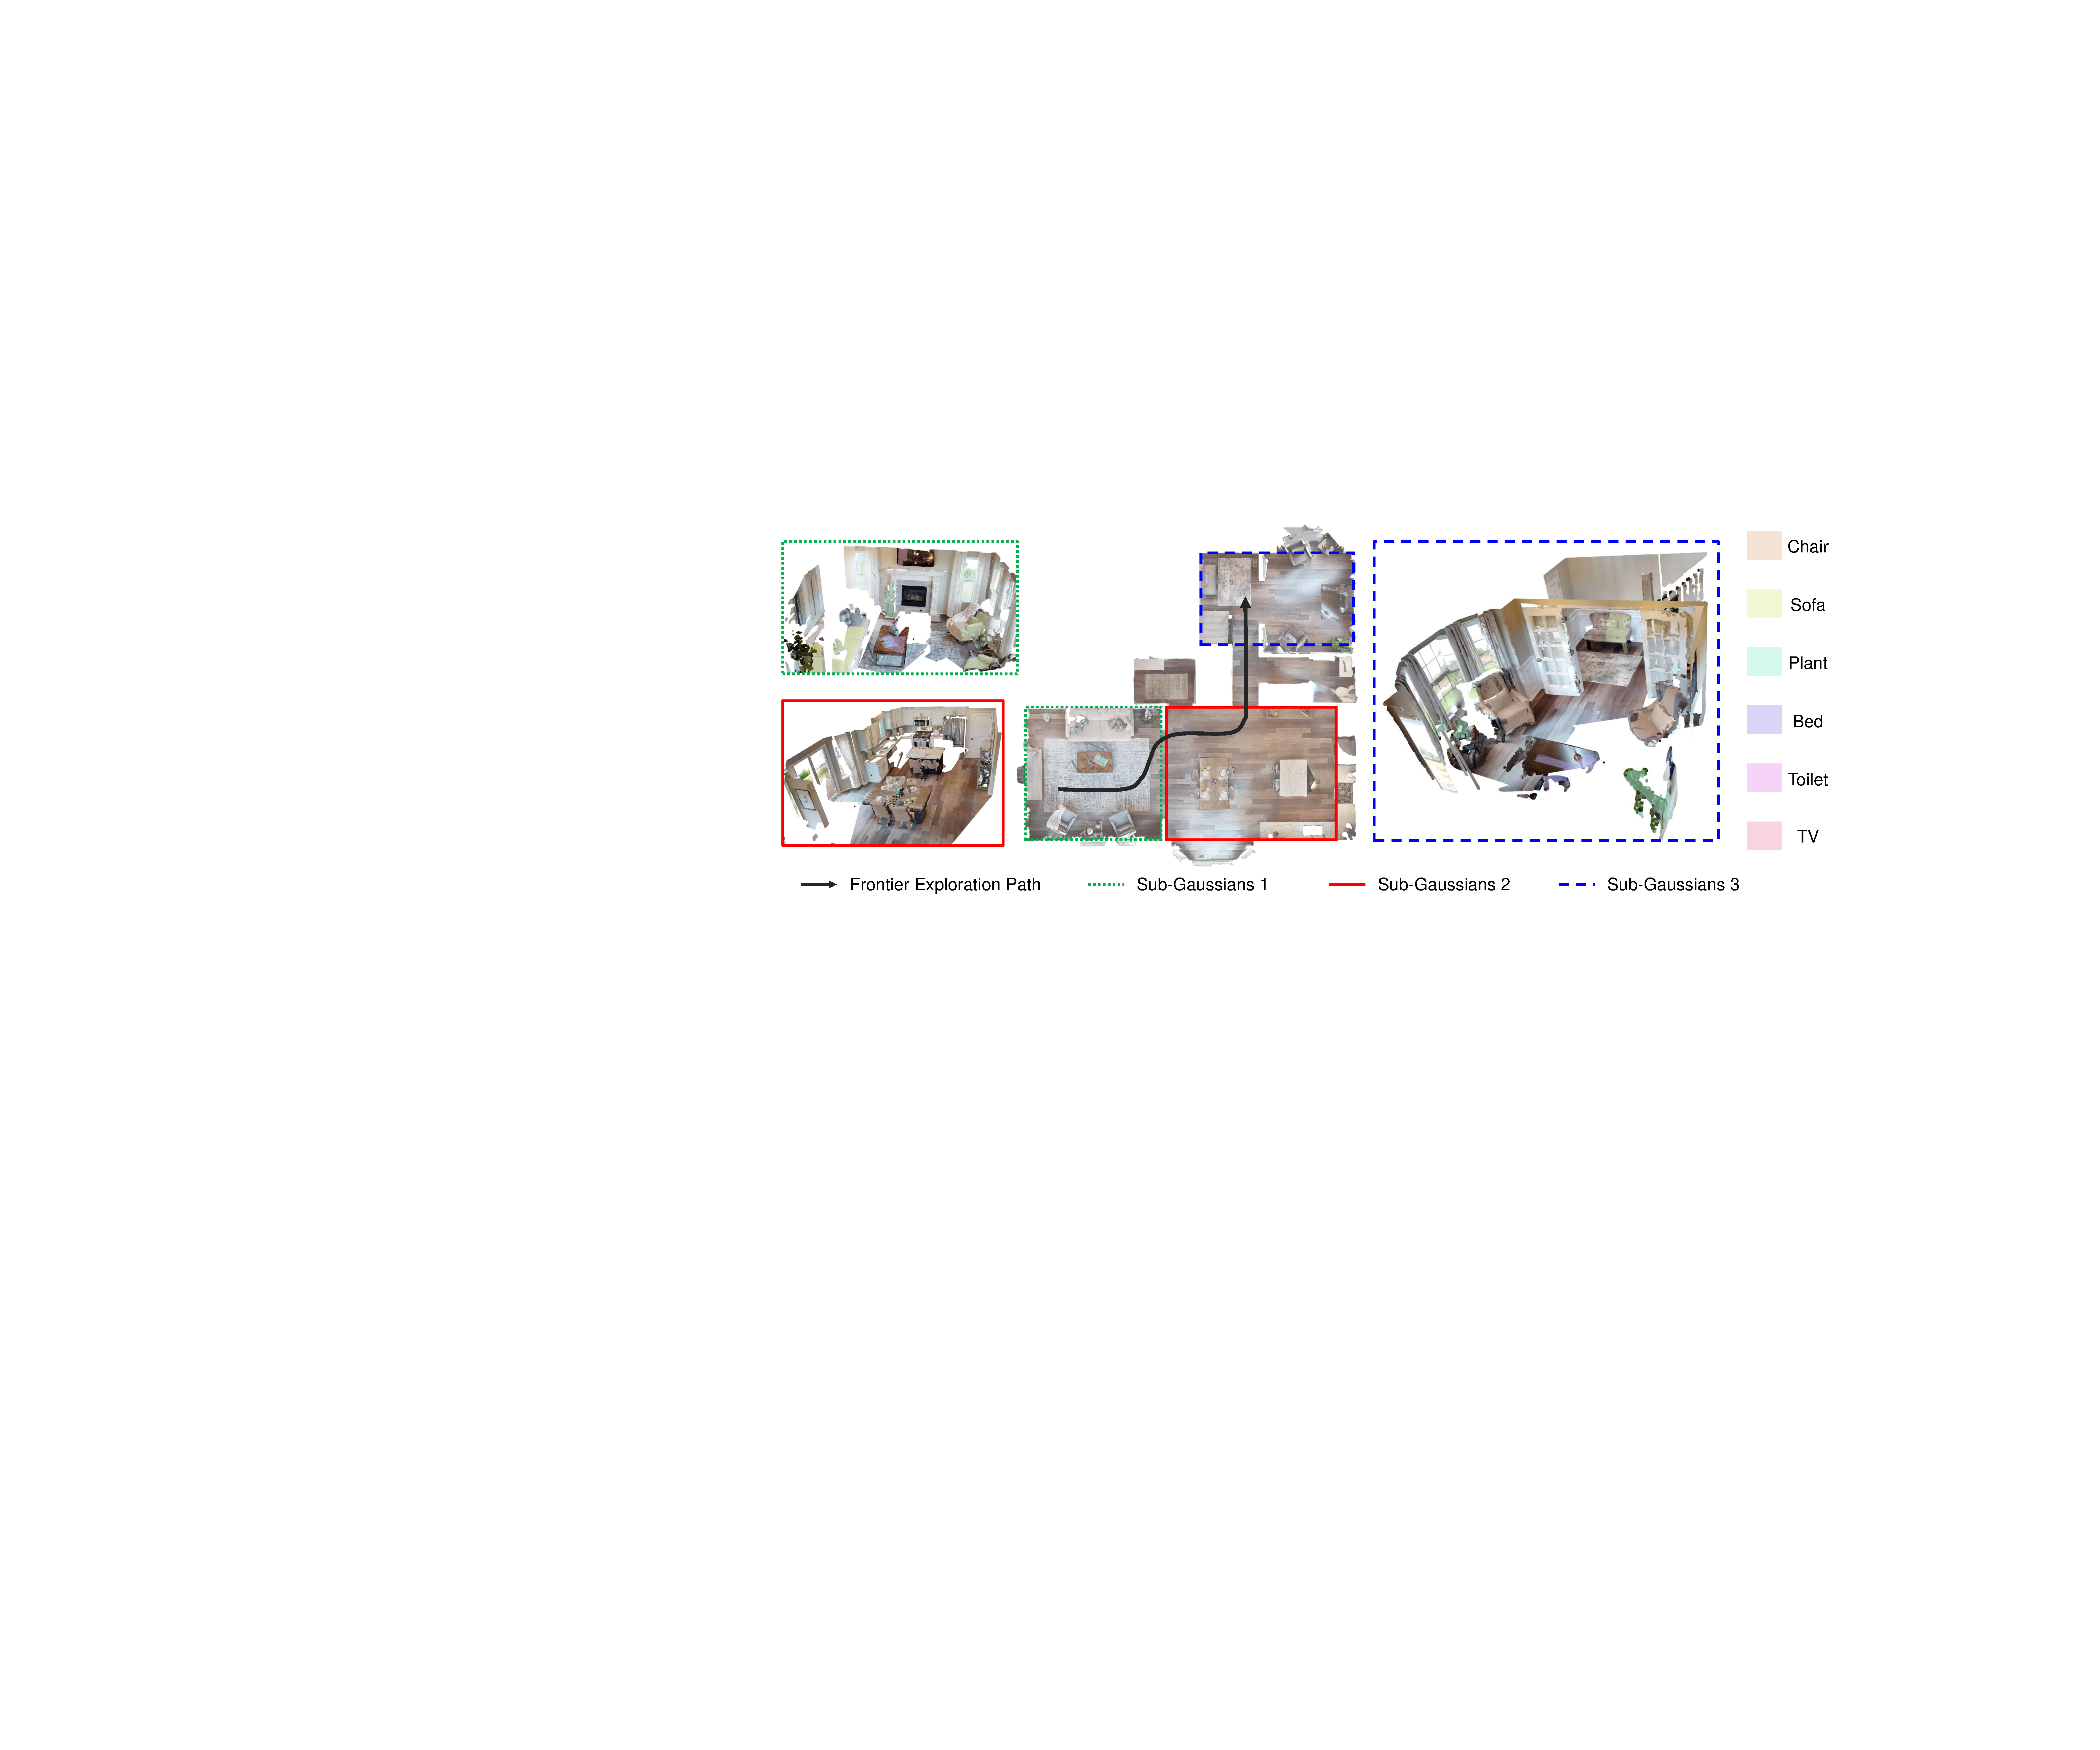
\includegraphics[width=0.95\linewidth]{pics/sub-gauss.pdf}
%   \caption{An Illustration of Sub-Gaussians Division. When initialized in an unkonwn environment, the agent first employs frontier exploration to explore the environment. The agent will next partition the collected observations into distinct subsets for constructing sub-Gaussians, in preparation for the subsequent Semantic Gaussian Construction.
%   }
%   \vspace{-16pt}
%   \label{fig:sub-gauss}
% \end{figure*}


\subsection{Overview}

In the IIN task, at the start of a new episode $e$, the agent is given a goal image $I_g$ that features a specified object instance $O_g$. The agent's goal is to navigate to the referred instance $O_g$ within the environment. At each timestep $t$, the agent acquires observations which include an RGB image $I_t$, a depth image $D_t$, and sensor pose reading $P_t$. Utilizing this information, the agent must decide upon and execute an action $a_t$. When calling stop action, the episode is considered successful only if the agent is within a certain range of the goal object.

To accomplish the IIN task, we propose a modular framework called Gaussian Splatting for Visual Navigation (GaussNav), as depicted in \Cref{fig:framework_overview}. In a new environment, the Instance ImageGoal Navitation in our proposed framework consists of three stages: Frontier Exploration, Semantic Gaussian Construction, as depicted in \Cref{fig:gauss_construct}, and Gaussian Navigation, illustrated in \Cref{fig:main}. Initially, during the first episode within an unknown environment, the agent employs frontier exploration to explore the environment and collect observations. We then use our proposed Semantic Gaussian to reconstruct the scene. Subsequently, in the following episodes, the agent leverages the Semantic Gaussian to ground the object instance $o$ depicted in the goal image and navigate to it. This process effectively transforms the IIN task into a more manageable PointGoal Navigation task.

\subsection{Frontier Exploration}

In the first episode of an unexplored environment, the agent simultaneously maintains two types of maps, an exploration map and an obstacle map, as illustrated in \Cref{fig:exp_obs_map}. The exploration map delineates the regions of the environment that have been explored, while the obstacle map marks the obstacles in the scene. By detecting the contours of the exploration map and excluding areas in the obstacle map, the agent sets the closest frontier point as a waypoint to facilitate exploration. The frontier-based exploration strategy is a well-established approach in robotics and autonomous navigation \cite{yamauchi1997frontier, holz2010evaluating}. It involves identifying the boundaries between the explored and unexplored regions of the environment, known as frontiers. The agent then selects the nearest accessible frontier point as its next target for exploration. This decision is based on the distance to the frontier, the navigability of the path, and the potential information gain from exploring that frontier \cite{julia2012comparison}. By iteratively exploring the nearest frontiers, the agent efficiently covers the entire environment while avoiding obstacles and previously explored areas. Through the application of this frontier-based exploration strategy, the agent collects observations of the entire environment.



\subsection{Semantic Gaussian Construction}

Our Semantic Gaussian is represented by a group of Gaussians, with each Gaussian characterized by a minimal set of nine parameters: a triplet for the RGB color vector $\mathbf{c}$, a triplet delineating the centroid $\bm{\mu} \in \mathbb{R}^3$, a scalar representing the radius $r$, a scalar quantifying the opacity $o \in [0,1]$, and a scalar representing the category label $l$. Different from original 3DGS \cite{kerbl3Dgaussians}, we simplify the representation of Gaussian by using only view-independent color and constraining the Gaussian to be isotropic. This simplification enhances computational efficiency while reducing memory requirements. For a comprehensive understanding of 3DGS \cite{kerbl3Dgaussians}, we highly recommend readers consulting the original paper \cite{kerbl3Dgaussians}. Our Semantic Gaussian Construction can be described as an iterative process comprising two alternating steps: Gaussian Densification and Semantic Gaussian Updating, as depicted in \Cref{fig:gauss_construct}. Gaussian Densification initializes new Gaussians in the Semantic Gaussian at each new incoming frame, while Semantic Gaussian Updating refines the parameters of each Gaussian through Differentiable Rendering.

\textit{Differentiable Rendering.} 3DGS \cite{kerbl3Dgaussians} renders an RGB image as follows: given a collection of 3D Gaussians and camera pose, first sort all Gaussians from front to back. RGB images can then be efficiently rendered by alpha-compositing the splatted 2D projection of each Gaussian in order in pixel space. The rendered color of pixel ${\bf p} = (u,v)$ can be written as:
\begin{equation}
\hat{I}(\mathbf{p}) = \sum_{i=1}^{n} \mathbf{c}_i f_i(\mathbf{p}) \prod_{j=1}^{i-1} (1 - f_j(\mathbf{p})),
\end{equation}
where $f_i(\bf{p})$ is computed as follows:
\begin{align}
    f(\mathbf{x}) = o \exp\left(-\frac{\|\mathbf{x} - \boldsymbol{\mu}\|^2}{2r^2}\right).\label{eq:gauss}
\end{align}
The $\boldsymbol{\mu}$ and $r$ are the splatted 2D Gaussians in pixel-space: 
\begin{equation}
    \boldsymbol{\mu}^{\textrm{2D}} = K \frac{E_t \boldsymbol{\mu}}{d}, \;\;\;\;\;\;
r^{\textrm{2D}} = \frac{f r}{d}, %
\quad \text{where} \quad d = (E_t \boldsymbol{\mu})_z.
\end{equation}
Here, $K$ is the camera's intrinsic matrix, $E_t$ embodies the extrinsic matrix that encodes the camera's rotation and translation at time $t$,  $f$ denotes the known focal length, and $d$ is the depth of the $i^{\text{th}}$ Gaussian relative to the camera's coordinate frame. 

\textbf{Render.} Different from 3DGS \cite{kerbl3Dgaussians}, we differentiably render depth and silhouette image, which determines the visibility and will be used for the next Gaussian Densification and Updating. The depth $D$ and silhouette image $S$ at pixel $\mathbf{p}$ is rendered as follows:
\begin{equation}
    \hat{D}(\mathbf{p}) = \sum_{i=1}^{n} d_i f_i(\mathbf{p}) \prod_{j=1}^{i-1} (1 - f_j(\mathbf{p})), 
\end{equation}
\begin{equation}
    \hat{S}(\mathbf{p}) = \sum_{i=1}^{n} f_i(\mathbf{p}) \prod_{j=1}^{i-1} (1 - f_j(\mathbf{p})).
\end{equation}
Above these, we also render the semantic segmentation results as follows:
\begin{equation}
    \hat{C}(\mathbf{p}) = \sum_{i=1}^{n} l_i f_i(\mathbf{p}) \prod_{j=1}^{i-1} (1 - f_j(\mathbf{p})).
\end{equation}

\textbf{Semantic Segmentation.} As depicted in \Cref{fig:gauss_construct}, the agent's RGB observation $I_t$ is segmented into $C_t$ using Mask-RCNN \cite{he2017mask}. The segmented result will be used for initializing new Gaussians in Gaussian Densification and supervising the Gaussians' parameters in Semantic Gaussian Updating. 


\textbf{Gaussian Densification.} Gaussian Densification is performed by comparing the rendered results at position $P_t$ using Gaussians from $t-1$ with the ground truth. This process adds new Gaussians where the previous Gaussians fail to represent the scene in the new observations. Following Keetha \etal \cite{keetha2023splatam}, we add new Gaussians based on a densification mask to determine which pixels should be densified:
\begin{equation}
\small
M(\textbf{p}) = \Bigl(\hat{S}(\textbf{p}) < 0.5\Bigr) + \Bigl( D(\textbf{p}) < \hat{D}(\textbf{p}) \Bigr) \Bigl(\textrm{L}_1\bigl(\hat{D}(\textbf{p})\bigr) > 50 \textrm{MDE} \Bigr),
\end{equation}
where the first term represents where the Semantic Gaussian is not adequately dense, and the second term indicates where the ground-truth depth is in front of the predicted depth and the depth error is greater than 50 times the median depth error (MDE).

\textbf{Semantic Gaussian Updating.}  After densifying current Semantic Gaussian, we update the parameters of Gaussians given poses and observations. This is done by differentiable-rendering and gradient-based-optimization, which is equivalent to the ``classic'' problem of fitting a radiance field to images with known poses. Specifically, we update the parameters of Gaussians by minimizing the RGB, depth and segmentation errors.



\begin{figure}[tb]
\centering
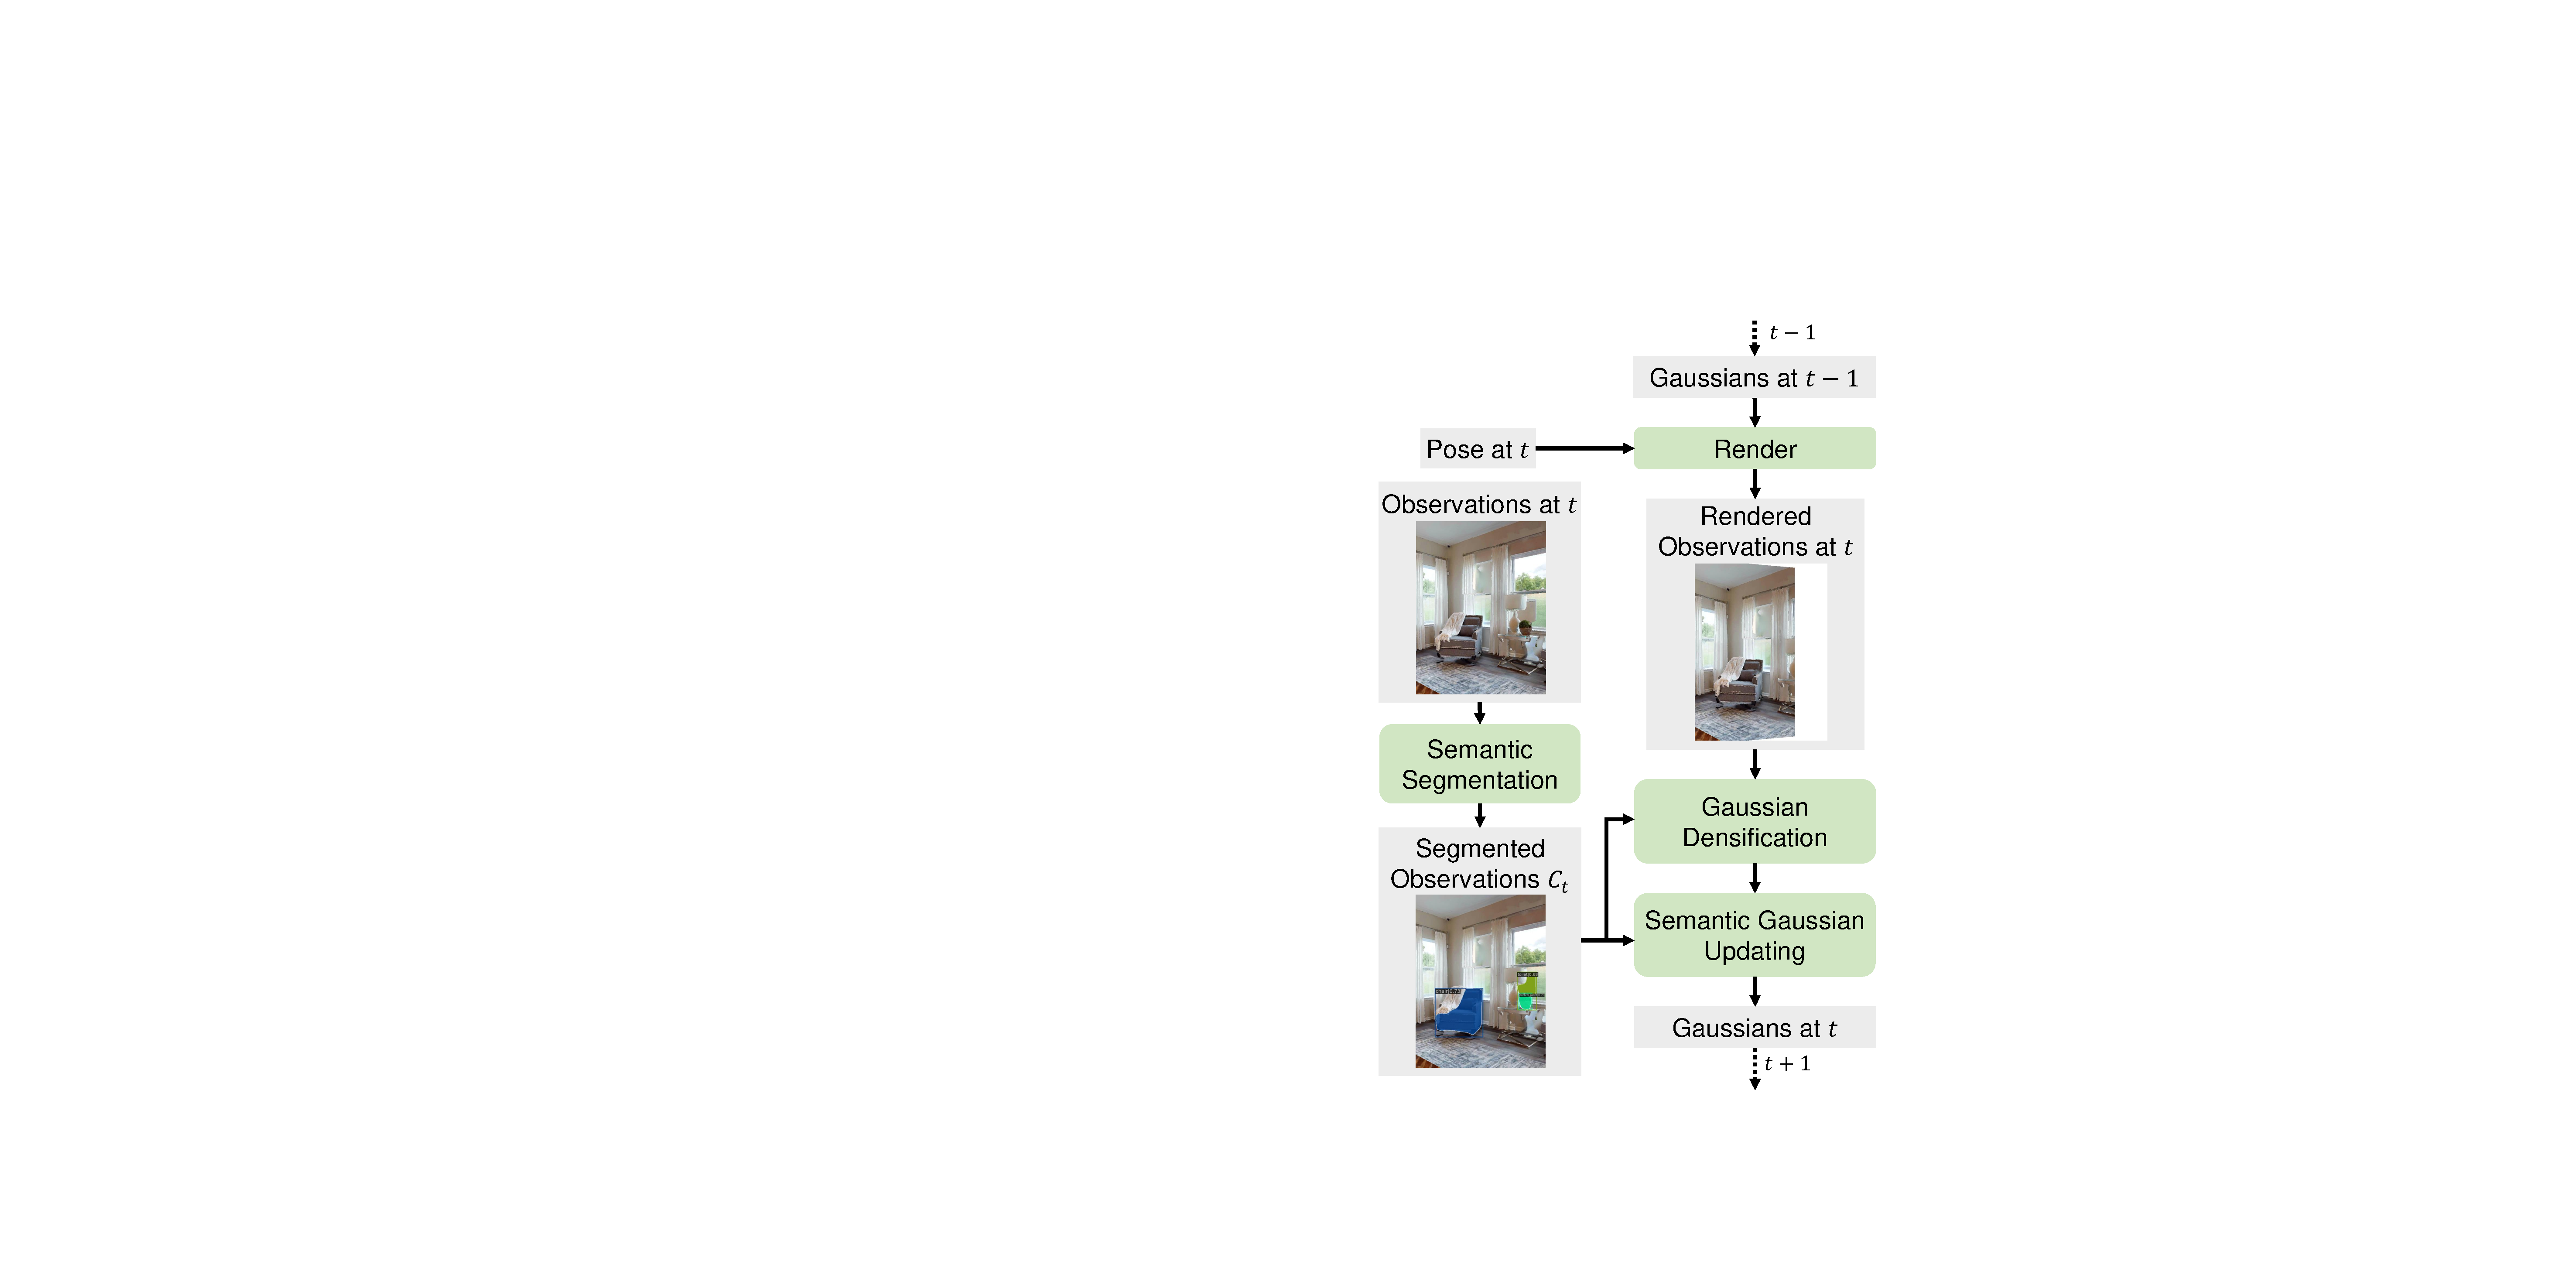
\includegraphics[width=0.8\linewidth]{pics/gauss_cons.pdf}
\caption{An illustration of Semantic Gaussian Construction. At timestep $t$, the pipeline updates the Gaussians from $t-1$ through densification and updating, which involves a comparison between the rendered RGB and depth images against the current input training views. Concurrently, semantic labels are assigned to the densified Gaussians using the segmented images. Finally, the Gaussians are refined through differentiable rendering.}
\label{fig:gauss_construct}
\vspace{-10pt}
\end{figure}

\begin{figure}[tb]
\centering
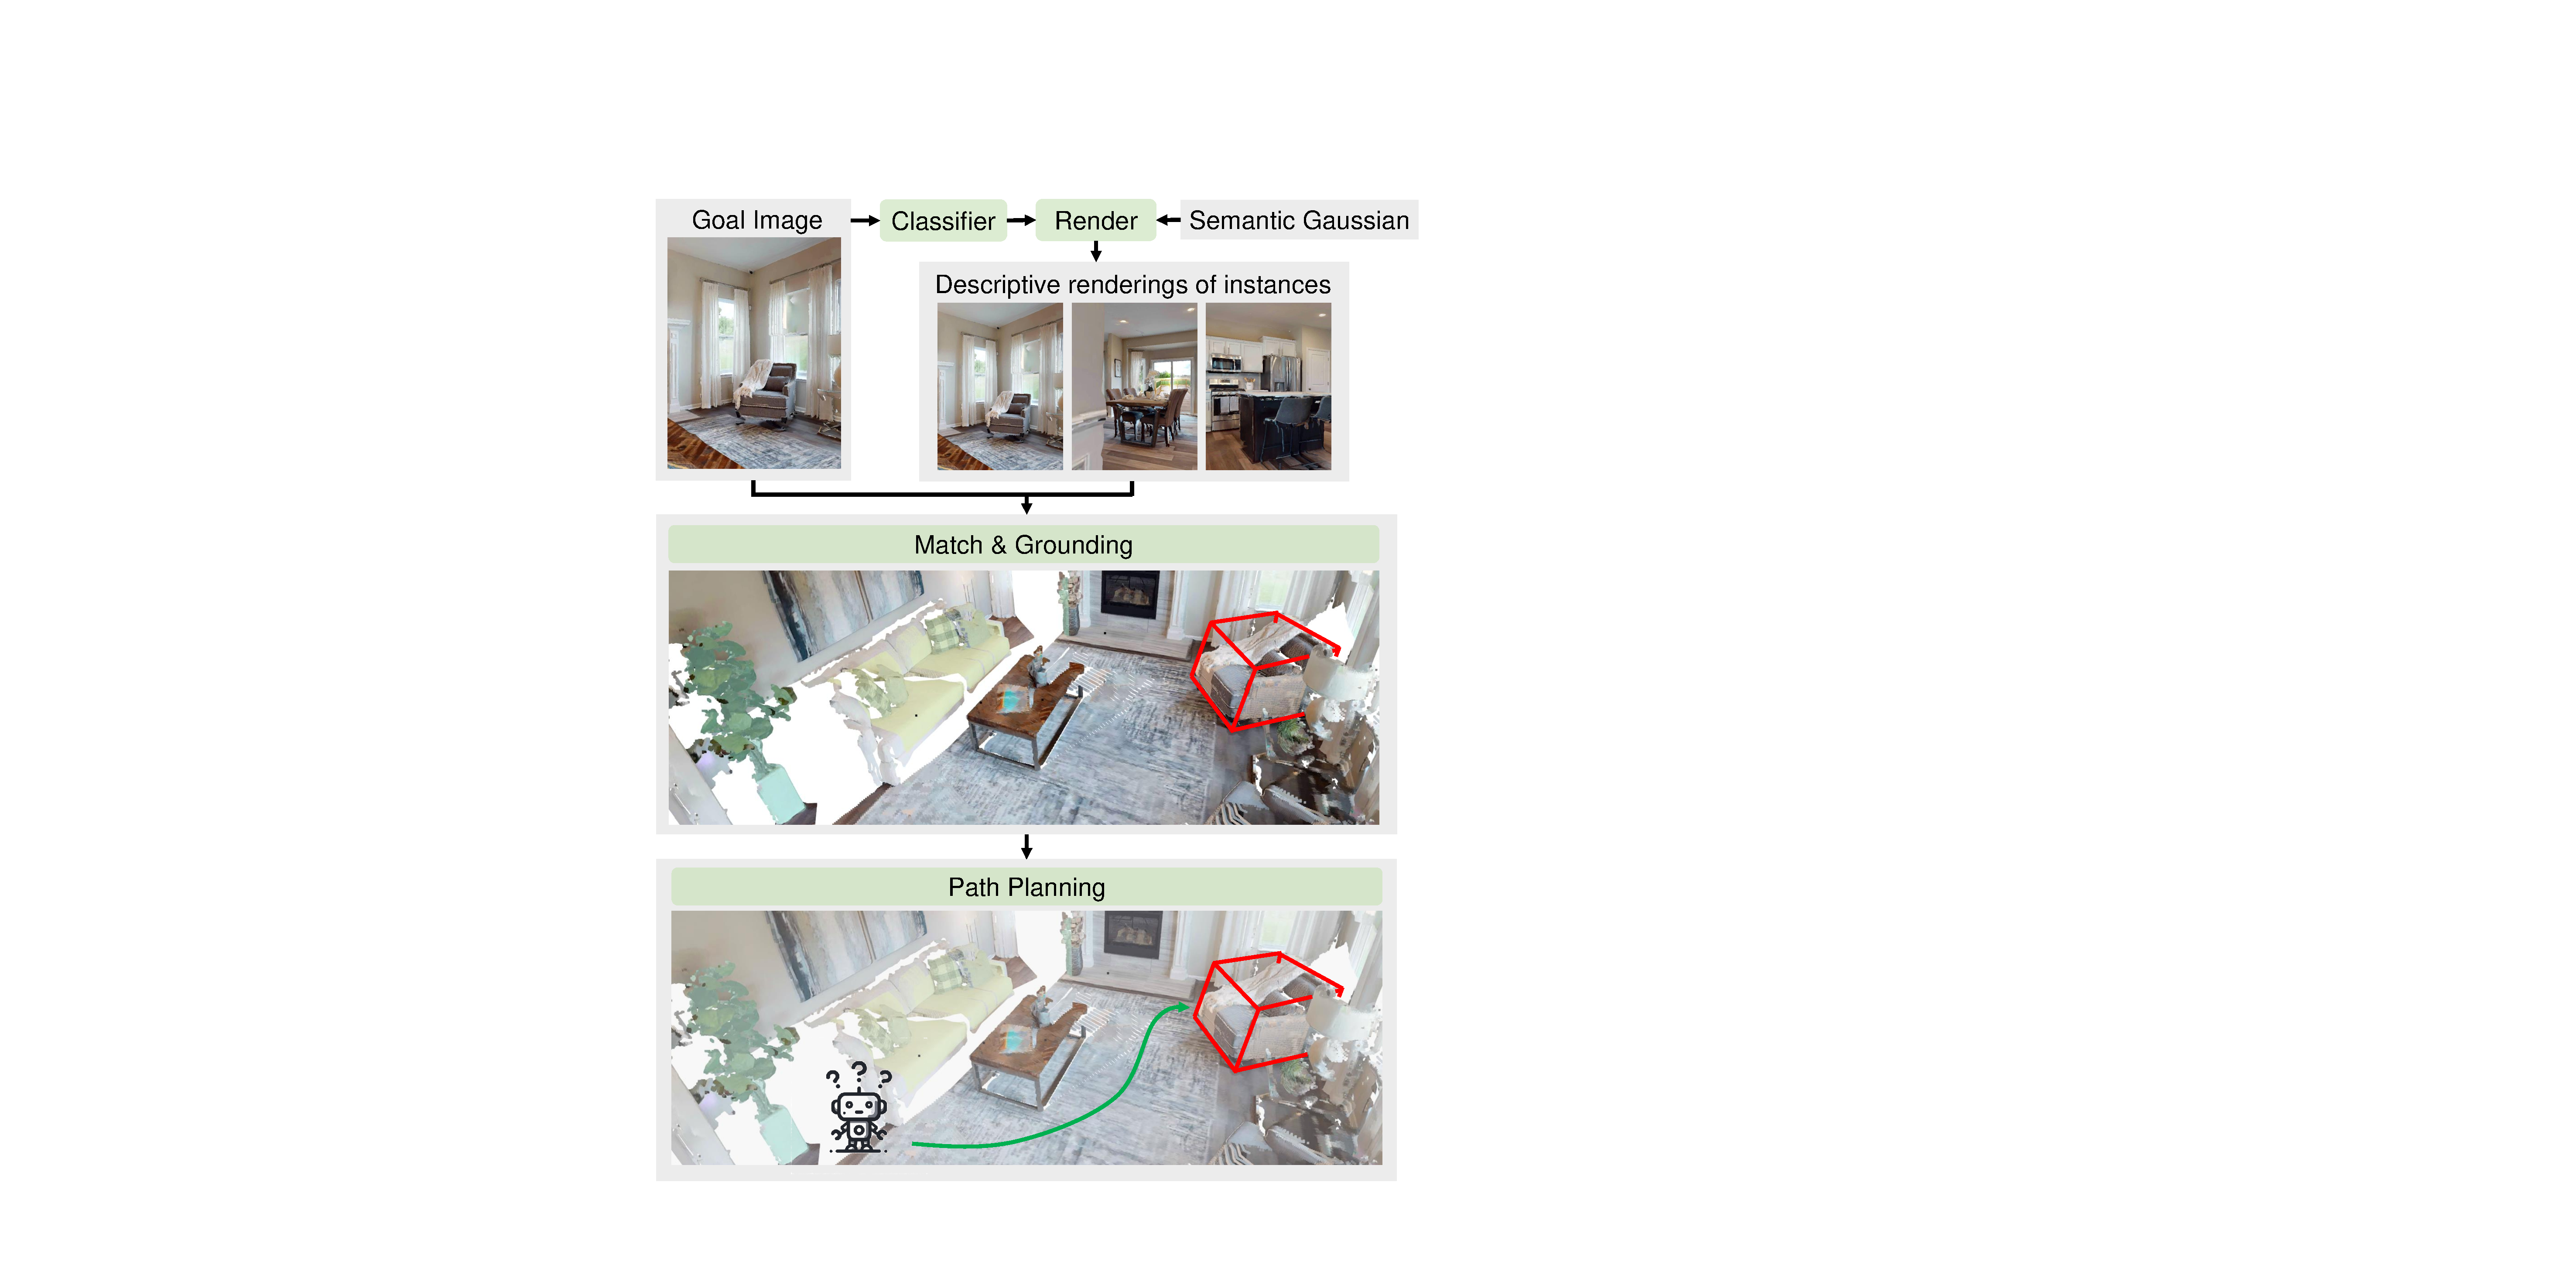
\includegraphics[width=0.9\linewidth]{pics/main.pdf}
\caption{An illustration of Gaussian Navigation. Our approach begins with the classification of the goal image using pre-constructed Semantic Gaussian. Upon determining the predicted class, we generate descriptive images around instances belonging to that class. These images are then matched with the target object to identify and ground the goal instance. Utilizing the map and the established goal, the agent employs path planning to compute the sequence of actions.}
\label{fig:main}
\vspace{-10pt}
\end{figure}




\subsection{Gaussian Navigation}

To navigate using a constructed Semantic Gaussian, we propose Gaussian Navigation, as illustrated in \Cref{fig:main}. We first classify the goal image $I_g$ to predict the semantic label $\hat{l}_g$ of the current target, such as `chair' in \Cref{fig:main}. This semantic label is then used to query the relevant Gaussians. For each relevant object instance of the same class, we render descriptive images. These renderings are compared with the goal image to ground the goal object, predicting its position $\hat{P}_g$. Finally, the Path Planning module generates a feasible path and determines the agent's action.

% Once the Semantic Gaussian is constructed and the agent's initial pose is known, transforming IIN into PointGoal Navigation requires: 1. converting the Semantic Gaussian into a map form that can be used for path planning, \textit{i.e.}, either 3D voxels $M_{3D}$ or 2D BEV grids $M_{2D}$, and 2. predicting the position of the target object instance $\hat{P}_g$. Therefore, we first convert the Semantic Gaussian into a point cloud, whereby each Gaussian is reduced to a single point in the point cloud representation. The point cloud is then voxelized into 3D voxels $M_{3D}$, then the 3D voxels $M_{3D}$ are projected to 2D BEV grids $M_{2D}$. By classifying and matching in the pre-built Semantic Gaussian $G_s$ with goal image $I_g$, we can ground target object's position $\hat{P}_g$, as depicted in \Cref{fig:main}. Given start pose $P_0$, predicted target object's position $\hat{P}_g$ and grid map $M_{2D}$, we can easily use Fast Marching Method (FMM) \footnote{\url{https://pythonhosted.org/scikit-fmm/}} to compute the shortest path and the corresponding action $a_t$.

\textbf{Classifier.} In IIN task, the agent receives an image depicting the target object $I_g$. However, comparing this image with renderings from navigable points within the entire scene becomes exceedingly time-inefficient due to the vastness of the search space. Consequently, with our Semantic Gaussian $G_s$, we only need to search for instances of the object category corresponding to the goal object. Therefore, we first classify the goal image $I_g$ into target category label $\hat{l}_g$. We use the goal images on the train split of HM3D-SEM \cite{yadav2023habitat} to finetune the image classification model, \textit{i.e.}, ResNet50 \cite{He2015}, pretrained on ImageNet \cite{5206848}. 

% In constrast, for better generalization in real world, there is no need to finetune the model.

\textbf{Match \& Grounding.} With the predicted target object's label $\hat{l}_g$, we identify all candidate objects that share the same class label. For each candidate instance, we generate a set of descriptive images by rendering the object from multiple viewpoints to capture its features. Specifically, for one training view containing possible candidate objects, we augment it to $n_v$ views by novel view synthesis (NVS). we denote the transformation from the camera to the world coordinate system of the training view as $\text{c2w}$, and record the translation of the potential target object in the camera frame as $\mathbf{t}^{o}_{c}$. We define the rotation matrix from the object to the world frame using the \textit{forward}, \textit{right}, and \textit{up} vectors. The \textit{forward} direction is the vector from the training view to the potential target object, namely $\mathbf{t}^{o}_{c}$. The \textit{up} direction is the vector $[0,\,-1,\,0]$, and the \textit{right} vector is orthogonal to both the \textit{forward} and \textit{up} vectors, forming a right-handed coordinate system with the \textit{right}, \textit{up}, and \textit{forward} vectors. The translation vector from the object to the world frame is
    \begin{equation}
        \mathbf{t}^{o}_{w} = \text{c2w} \times \mathbf{t}^{o}_{c}.
        \label{equ:NVS0}
\end{equation}
Together, the rotation matrix and translation vector constitute the rigid transformation matrix $\text{o2w}$ from the object to the world frame.


We define the rotation matrices around the $y$-axis and $x$-axis as $\mathbf{R}_y(\theta)$ and $\mathbf{R}_x(\theta)$, respectively, representing new viewpoints formed by rotating around the object by an angle $\theta$ in the horizontal and vertical directions. Thus, the transformation from the camera to the world frame for new viewpoints in the horizontal direction is
\begin{equation}
    \text{c2w}_h(\theta) = \text{o2w} \times \mathbf{R}_y(\theta) \times \text{w2o} \times \text{c2w},
    \label{equ:NVS1}
\end{equation}
and in the vertical direction:
\begin{equation}
    \text{c2w}_v(\theta) = \text{o2w} \times \mathbf{R}_x(\theta) \times \text{w2o} \times \text{c2w}.
    \label{equ:NVS2}
\end{equation}
In experiments, when $n_v=1$, we do not perform NVS; when $n_v=3$, we perform NVS at $\theta = \pm15^\circ$ (both horizontal and vertical); and when $n_v=5$, we use $\theta = \pm15^\circ$, $\pm30^\circ$.


After NVS, the original training views are augmented. The augmented rendering set for the $i$-th object instance is denoted as $S_i$. Let $n$ denote the observed instances of the same class as target object, then the universal set of $S$ can be formulated as:
\begin{equation}
    S = \{S_1, S_2, \ldots, S_n\}  \quad \text{for} \quad i=1,2,\ldots,n.
\end{equation}
To distinguish the target object from these candidates, we can formulate the question as:
\begin{equation}
\begin{split}
      i_{\text{max}} = arg\max \{ \max_{s \in S_1} \Omega (s), \max_{s \in S_2} \Omega (s), \ldots, \max_{s \in S_n} \Omega (s) \} \\
      \text{for} \quad i=1,2,\ldots,n,
    \label{eq:match}  
\end{split}
\end{equation}
where $\Omega (\cdot)$ is defined as the matched number of keypoints between renderings and goal image $I_g$. Specifically, for the rendering $s \in S_i$ of the $i$-th object instance and the goal image $I_g$, we extract the pixel-wise $(x, y)$ coordinates of the keypoints and their associated feature descriptors $V_t$ using DISK \cite{tyszkiewicz2020disk}. That is:
\begin{equation}
(K_t, V_t) = \text{DISK}(s), \quad (K_g, V_g) = \text{DISK}(I_g).
\label{eq:feature1}
\end{equation}
Subsequently, the matched pairs $(\hat{K_t}, \hat{K_g})$ are computed using LightGlue \cite{lindenberger2023lightglue}. The feature matching process is formulated as follows:
\begin{equation}
(\hat{K_t}, \hat{K_g}) = \text{LightGlue}((K_t, V_t), (K_g, V_g)).
\label{eq:matching}
\end{equation}
Thus, the number of matched points, \textit{i.e.}, the length of $\hat{K_t}$ or $\hat{K_g}$, is denoted as $\Omega$. The candidate object whose rendered images yield the highest number of matched keypoints is then selected as the target object, as shown in \Cref{eq:match}. 


When the object instance is selected, we ground the object in the Semantic Gaussian. Due to the presence of outliers, which are caused by errors in semantic segmentation, we perform clustering on the instances on the map. Specifically, we use Density-based Spatial Clustering of Applications with Noise (DBSCAN) \footnote{\url{https://scikit-learn.org/stable/modules/generated/sklearn.cluster.DBSCAN.html}}, which groups together points that are closely packed together, marking as outliers points that lie alone in low-density regions. With the precise selected object instance's location, we can easily transform the IIN task to a PointGoal task.


\textbf{Path Planning.} The Semantic Gaussian is not designed for path planning. We first convert the Semantic Gaussian into a point cloud, whereby each Gaussian is reduced to a single point in the point cloud representation. The point cloud is then voxelized into 3D voxels $M_{3D}$, then the 3D voxels $M_{3D}$ are projected to 2D BEV grids $M_{2D}$. Here, we use the 2D projection of Semantic Gaussian rather than the 2D geometric map used in pre-exploration to maintain a consistent representation throughout the pipeline. Our Semantic Gaussian initializes Gaussians using point cloud derived from depth image and does not prune any Gaussian in the optimization stage. Thus, 2D projection of Semantic Gaussian or 2D geometric map are fundamentally equivalent.

Given 2D BEV grid map $M_{2D}$, along with the agent's starting position and the goal's location, we can efficiently generate a shortest distance field using FMM. Each point within this field encapsulates the minimal distance necessary to traverse from the starting point to the goal.  We extract a relevant subset of this distance field that falls within the agent's operational range. Subsequently, a waypoint is chosen from this subset to ensure it avoids any intersections with obstacles while adhering to a local minimum in the distance field. With the selected waypoint, the agent can readily calculate an action based on the angle and distance from its current state. The agent iterates the aforementioned process to generate a sequence of actions, continuing until the destination is reached.



